% Rešerše – Fakturoid (vkládá se do kapitoly 01-reserse.tex)
\section{Fakturoid}\label{sec:reserse-fakturoid}

Fakturoid je česká online fakturační služba určená především živnostníkům a~malým firmám. Základní údaje shrnuje tabulka~\ref{tab:reserse-fakturoid}.

\begin{table}[H]
\centering
\small
\begin{tabular}{>{\raggedright\arraybackslash}p{0.24\linewidth}>{\raggedright\arraybackslash}p{0.70\linewidth}}
\hline
\textbf{Kritérium} & \textbf{Zjištění} \\
\hline
Název & Fakturoid \\
Společnost & Fakturoid s.r.o., Praha (CZ); založili Lukáš Konarovský a~Jan Korbel, v~provozu od prosince 2009 \cite{fakturoid-onas} \\
Typ aplikace & webová aplikace (responzivní) a~mobilní aplikace pro iOS a~Android \cite{fakturoid-tarify2025,fakturoid-srovnani} \\
Hostování & pouze cloud (SaaS provozovaný výrobcem); vlastní server ani lokální instalace nejsou možné \\
Licence & proprietární, předplatné \\
Cena & ceny s~DPH při měsíční platbě, roční platba je přibližně o~8~\% levnější: Zdarma 0~Kč (1 uživatel, nejvýše 5 odběratelů), Na lehko 199~Kč, Na každý den 279~Kč, Na maximum 519~Kč měsíčně; další uživatel 120~Kč měsíčně; začínající podnikatelé mají první rok slevu 50~\% \cite{fakturoid-tarify2025,fakturoid-srovnani,fakturoid-cenik} \\
Zkušební verze & 30 dní se všemi funkcemi a~tři veřejné demoverze bez registrace \cite{fakturoid-srovnani} \\
\hline
\end{tabular}
\caption{Základní údaje o~řešení Fakturoid}\label{tab:reserse-fakturoid}
\end{table}

\subsection{Zkušenosti ze zkušební verze}

Celkový vzhled aplikace je minimalistický a~přehledný. Detail faktury zobrazuje všechny podstatné údaje na jedné obrazovce bez nutnosti posouvat stránku a~seznam faktur ukazuje jen nejdůležitější údaje, přičemž podrobnosti se zobrazí až po otevření dokladu. Stejně jako v~navrhované aplikaci lze při vystavování dokladu vybrat existujícího odběratele, nebo rovnou založit nového. Detail kontaktu zobrazuje kromě údajů zákazníka i~všechny doklady, které jsou s~ním spojené. Užitečná je také \emph{soukromá poznámka} u~dokladu, kterou zákazník nevidí, a~webová faktura, tedy odkaz, přes který si zákazník může doklad prohlédnout, zaplatit nebo stáhnout ve formátu PDF či ISDOC.

Formulář faktury obsahuje tlačítko \emph{Zobrazit náhled}, které v~okně nad formulářem zobrazí výslednou fakturu a~umožní ji z~náhledu rovnou vystavit (obrázek~\ref{obr:fakturoid-nahled}). Náhled se však nezobrazí, dokud není vyplněn odběratel; aplikace místo něj zobrazí pouze hlášení o~chybějícím povinném údaji. Z~pohledu uživatele by bylo vhodnější náhled zobrazit vždy a~na chybějící údaje jen upozornit.

\begin{figure}[H]
\centering
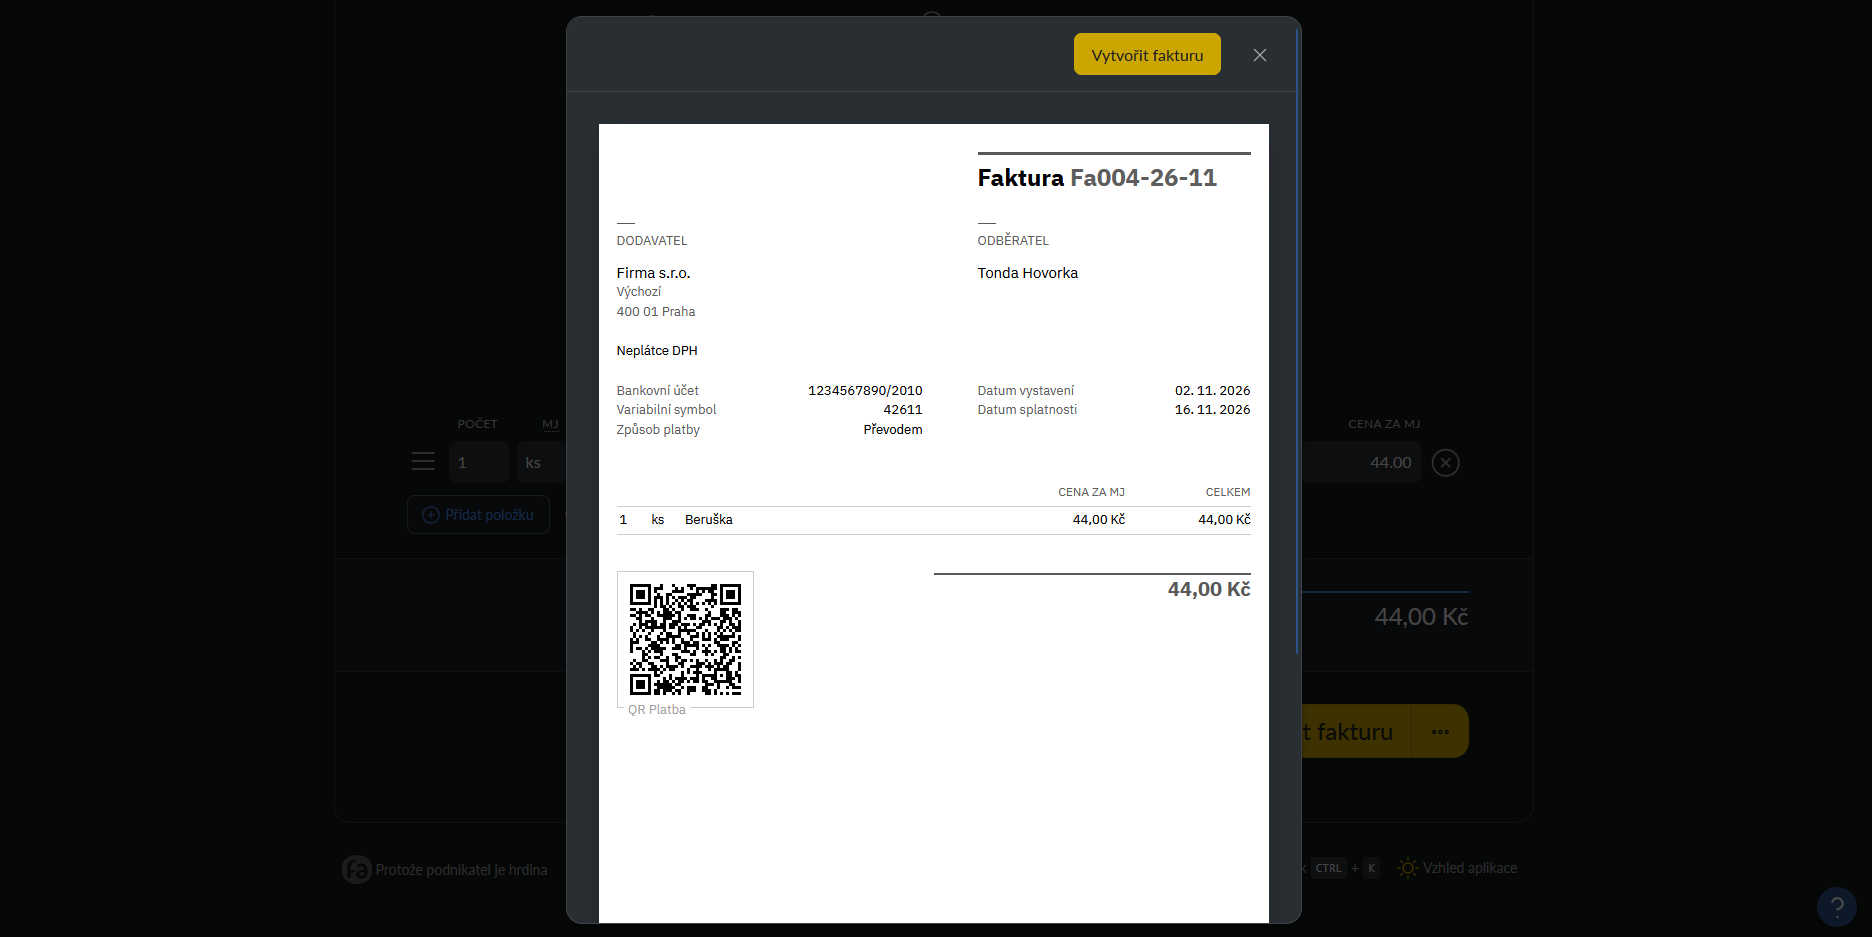
\includegraphics[width=0.85\linewidth]{obrazky/reserse/fakturoid_nahled_faktury.png}
\caption{Náhled faktury před jejím vystavením v~aplikaci Fakturoid (zdroj: vlastní snímek obrazovky ze zkušební verze, pořízeno 2.~11.~2026)}\label{obr:fakturoid-nahled}
\end{figure}

Řada prvků rozhraní je však nejasná. Cenové nabídky, šablony i~ceník jsou umístěny jako podzáložky v~sekci \emph{Faktury}. Šablony přitom neslouží ke změně vzhledu dokumentu, jak by název napovídal, ale k~uložení předvyplněné faktury pro opakované použití, a~pro nabídky nejsou k~dispozici vůbec. Vzhled dokumentu lze vybrat pouze ze šesti předdefinovaných variant. Po přechodu do ceníku se změní celá horní lišta a~uživatel ztratí přímý přístup k~fakturám a~nabídkám, aniž by mu rozhraní jasně ukázalo, ve které části aplikace se nachází. Stejné funkce jsou navíc dostupné z~více míst (z~tlačítka \enquote{+}, z~nabídky pod třemi tečkami a~z~hlavní navigace). Rušivě působí výrazná oznámení v~rámečku uprostřed obrazovky, která se zobrazují po každé akci, a~nápověda k~rychlým akcím, kterou se nepodařilo zavřít.

Přepsání čísla nabídky na vlastní tvar (například \texttt{NAB001-26}) formulář sice povolí, ale při uložení jej odmítne, protože neodpovídá formátu nastavenému pro číselnou řadu. Formát se nastavuje pomocí zástupných znaků, což je pro běžného uživatele zbytečně složité. Změnu jediného výchozího údaje, například splatnosti, nelze provést samostatně, ale jen přes celý formulář nastavení faktury. Nová ceníková položka se ve výchozím stavu zakládá jako skladová s~povinným množstvím, nákupní a~prodejní cenou, což servisní firma bez skladu nepotřebuje. Správa uživatelů a~oprávnění nebyla ve zkušební verzi dostupná.

Ve srovnání s~navrhovanou aplikací Fakturoid neobsahuje evidenci zakázek, zařízení ani provedené práce, materiál eviduje pouze formou skladu, neumožňuje vlastní šablony dokumentů a~místo kalendáře nabízí jen přehled a~statistiky. Cenové nabídky, sklad s~pohyby, upomínky a~více číselných řad jsou navíc dostupné až v~nejdražším tarifu \cite{fakturoid-srovnani}.

\subsection{Vhodnost pro malé firmy}

Fakturoid je velmi vhodný pro živnostníky a~malé firmy, které potřebují především rychle vystavovat faktury: nic se neinstaluje ani nespravuje, cena je nízká a~rozhraní přehledné. Servisní firma by však pokryla jen fakturační konec svého procesu a~evidenci zakázek by musela vést jinde. Data jsou uložena výhradně v~cloudu výrobce.
